\subsection{Constructing Confidence Intervals}

\underline{Problem:} Given data sampled with mean $\mu = (\mu_1, \dots, \mu_m)$, we want to identify the largest $\mu_j$ (1) and perform inference on this $\mu_j$ (2).

\noindent \textbf{Binary data} $\mu_j \rightsquigarrow p_j \in (0,1)$. Can arise in different settings:
\begin{enumerate}
    \item $X_j \sim \text{Binom}(n, p_j)$ independently for $j=1..m$ (e.g., trials for medications).
    \item $X \sim \text{Multinom}(n, p=(p_1 \dots p_m))$ (e.g., $n$ voters who vote for one candidate $j=1..m$).
\end{enumerate}

\noindent \textbf{Goal for today:} One-sided confidence interval for $p_{\hat{j}}$. $\hat{L}_{\hat{j}}(X) \le p_{\hat{j}}$ with confidence $\ge 1-\alpha$.

\emph{\textbf{Methods to construct CI}}
\begin{enumerate}
    \item Data-splitting: choose $J$ as a function of half the data \& construct CI using the rest of the data.
    \item Multiplicity correction.
    \item Selective inference condition on selection event (value of $J$).
    \item Randomized inference.
\end{enumerate}
\begin{center}
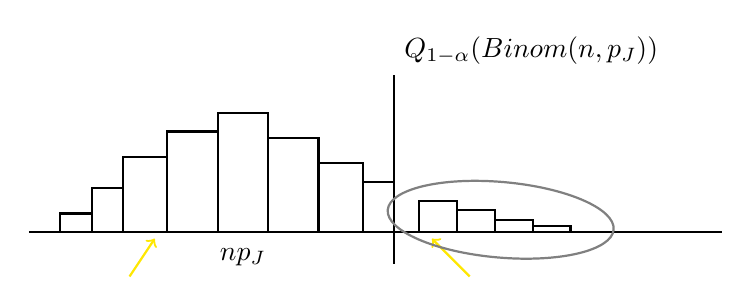
\begin{tikzpicture}[scale=0.8, every node/.style={scale=1}]

    % Horizontal axis
    \draw[thick] (0,0) -- (11,0);

    % Histogram bars
    \draw[thick] (0.5,0) rectangle (1.0, 0.3);
    \draw[thick] (1.0,0) rectangle (1.5, 0.7);
    \draw[thick] (1.5,0) rectangle (2.2, 1.2);
    \draw[thick] (2.2,0) rectangle (3.0, 1.6);
    \draw[thick] (3.0,0) rectangle (3.8, 1.9); % Peak
    \draw[thick] (3.8,0) rectangle (4.6, 1.5);
    \draw[thick] (4.6,0) rectangle (5.3, 1.1);
    \draw[thick] (5.3,0) rectangle (5.8, 0.8);
    
    % The right tail bars
    \draw[thick] (6.2,0) rectangle (6.8, 0.5);
    \draw[thick] (6.8,0) rectangle (7.4, 0.35);
    \draw[thick] (7.4,0) rectangle (8.0, 0.2);
    \draw[thick] (8.0,0) rectangle (8.6, 0.1);

    % Vertical quantile line
    \draw[thick] (5.8, -0.5) -- (5.8, 2.5) node[above right] {$Q_{1-\alpha}(\text{Binom}(n,p_J))$};

    % Mean label np_J
    \node at (3.4, -0.4) {$np_J$};

    % Yellow arrows
    \draw[->, thick, yellow!90!orange] (1.6, -0.7) -- (2.0, -0.1);
    \draw[->, thick, yellow!90!orange] (7.0, -0.7) -- (6.4, -0.1);

    % Hand-drawn circle around the tail
    \draw[thick, gray, rotate around={-5:(7.5,0.3)}] (7.5, 0.2) ellipse (1.8cm and 0.6cm);

\end{tikzpicture}
\end{center}

\vspace{0.5cm}

\begin{align*}
    \hat{L}_J(X) &= \inf \{ t \in [0,1] : X \le Q_{1-\alpha}(\text{Binom}(n,t)) \} \\
    \mathbb{P}\{ \hat{L}_J(X) \le p_J \} &\ge \mathbb{P}\{ X \le Q_{1-\alpha}(\text{Binom}(n,p_J)) \} \\
    &\ge 1 - \alpha
\end{align*}

\begin{enumerate}
    \item Data-Splitting. $n = n_0 + n_1$. $X_{i,j} \sim \text{Ber}(p_j)$ for $i=1.,\dots, n, \ j=1,\dots, m$.
\begin{align*}
    J &= \arg\max_{j=1..m} \sum_{i=1}^{n_0} X_{ij} \\
    \hat{L}_J(X) &= \inf \left\{ t : \sum_{i=n_0+1}^n X_{ij} \le Q_{1-\alpha}(\text{Bin}(n_1, t)) \right\}
\end{align*}
Valid because $\sum_{i=n_0+1}^n X_{iJ} \mid J \sim \text{Bin}(n_1, p_J)$.

\item Multiplicity correction. $J = \arg\max_j \left( \sum_{i=1}^n X_{ij} \right)$.
\[ \hat{L}_J(X) = \inf \left\{ t : \sum_{i=1}^n X_{iJ} \le Q_{1-\frac{\alpha}{m}}(\text{Bin}(n, t)) \right\} \]

\noindent \textbf{Proof:}
\begin{align*}
    \mathbb{P} \{p_J < \hat{L}_J(X)\} &\le \mathbb{P} \{p_j < \hat{L}_j(X) \text{ for some } j=1..m\} \\
    &\le \sum_{j=1}^m \mathbb{P} \{p_j < \hat{L}_j(X)\} \\
    &\le m \cdot \frac{\alpha}{m} = \alpha
\end{align*}

\item Selective Inference. $\longrightarrow$ also condition on $X_k \ \forall k \neq j$.

\[ X_J \mid \dots \sim \text{TruncBinom}\left(n, p_J, \left[1+\max_{k \neq j} X_k, n\right]\right) \]

\begin{center}
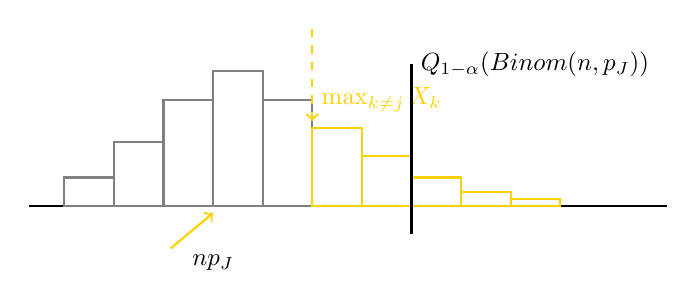
\begin{tikzpicture}[scale=0.9, every node/.style={scale=0.9}]
    % Horizontal axis
    \draw[thick] (0,0) -- (9,0);

    % Standard bars (before truncation)
    \draw[thick, gray] (0.5,0) rectangle (1.2, 0.4);
    \draw[thick, gray] (1.2,0) rectangle (1.9, 0.9);
    \draw[thick, gray] (1.9,0) rectangle (2.6, 1.5);
    \draw[thick, gray] (2.6,0) rectangle (3.3, 1.9);
    \draw[thick, gray] (3.3,0) rectangle (4.0, 1.5);

    % Highlighted bars (truncated support)
    \draw[thick, yellow!70!orange] (4.0,0) rectangle (4.7, 1.1);
    \draw[thick, yellow!70!orange] (4.7,0) rectangle (5.4, 0.7);
    \draw[thick, yellow!70!orange] (5.4,0) rectangle (6.1, 0.4);
    \draw[thick, yellow!70!orange] (6.1,0) rectangle (6.8, 0.2);
    \draw[thick, yellow!70!orange] (6.8,0) rectangle (7.5, 0.1);

    % Truncation indicator
    \draw[->, dashed, yellow!70!orange, thick] (4.0, 2.5) -- (4.0, 1.2) node[above right] {$\max_{k \neq j} X_k$};

    % Mean annotation
    \draw[->, thick, yellow!70!orange] (2.0, -0.6) -- (2.6, -0.1);
    \node at (2.6, -0.8) {$np_J$};

    % Quantile Line
    \draw[thick] (5.4, -0.4) -- (5.4, 2.0) node[right] {$Q_{1-\alpha}(\text{Binom}(n, p_J))$};
\end{tikzpicture}
\end{center}

\[ \hat{L}_J(X) = \inf \left\{ t : \sum_{i=1}^n X_{iJ} \le Q_{1-\alpha}\left(\text{TruncBin}(n, t, 1+\max_{k \neq j} X_k, n)\right) \right\} \]


\item Randomized Inference. 
Let $\tilde{X}_j = X_j + \mathcal{N}(0, \sigma^2)$ \quad (where $X_j = \sum_{i=1}^n X_{ij}$).

\[ J = \operatorname*{argmax} \tilde{X}_j \]

\noindent $X_J \mid \tilde{X}_J$ has PMF proportional to:
\[ \propto \binom{n}{x} p_J^x (1-p_J)^{n-x} \cdot e^{-\frac{(\tilde{X}_J - x)^2}{2\sigma^2}} \]

\noindent \textit{Mote:} $(X_j, \tilde{X}_j) \perp\!\!\!\perp X_k, \tilde{X}_k \ \forall k \neq j$. \\
i.e. this is the conditional distribution of $X_J \mid \tilde{X}_J, (\tilde{X}_k)_{k \neq j}, J$.

$J = \arg\max_j \left( \sum_{i=1}^n X_{ij} \right)$.

Using the Tilted Binomial distribution $(n, p_J; \tilde{X}_J, \sigma^2)$:
$$ \hat{L}_J(X) = \inf \left\{ t : X_J \le Q_{1-\alpha}(\text{TiltedBinom}(n, t; \tilde{X}_J, \sigma^2)) \right\} $$

\end{enumerate}


